%! Author = Len Washington III
%! Date = 11/05/2023

% Preamble
\documentclass[12pt]{report}

\usepackage[12]{cs430recitation}

% Document
\begin{document}

%<*Recitation-12>
\subsection{After Lecture 21 \& 22 \& 23}~\\
Practice Problems (all taken from previous exams)
\begin{enumerate}
	\item The number of trees in a binomial heap with $n$ nodes is
	\begin{enumerate}
	    \item $\log n$
	    \item $n$
	    \item $n\log n$
	    \item $\frac{n}{2}$
	\end{enumerate}
	\item Which two Fibonacci heap functions have the same complexity?
	\begin{enumerate}
	    \item \Call{Insertion}{}, \Call{Union}{}
	    \item \Call{Insertion}{}, \Call{Deletion}{}
	    \item \Call{ExtractMin}{}, \Call{Insertion}{}
	    \item \Call{Union}{}, \Call{Delete}{}
	\end{enumerate}
	\item If $V$ is the total number of elements, in the worst case, how many leader pointer updates are needed when fusing two groups in the union method:
	\begin{enumerate}
	    \item $O(1)$
		\item $O(\log|V|)$
		\item $O(|V|)$
		\item $O\left(|V|^{2}\right)$
	\end{enumerate}
	\item Consider the following program: \lstinputlisting[language=Python,label={lst:12-py}]{12_4.py}
	Assume the disjoint set data structure is implemented so after a union,
	the smallest valued element in the set is the label of the set.
	What is the output?
	\begin{enumerate}
	    \item 6~~3~11~9
		\item 3~~1~~1~3
		\item 1~~3~~3~1
		\item 9~11~11~9
	\end{enumerate}
	\item Show the Fibonacci heap that results from calling \Call{FIB-HEAP-EXTRACT-MIN}{} on the Fibonacci heap shown
	\begin{figure}[H]
		\centering
		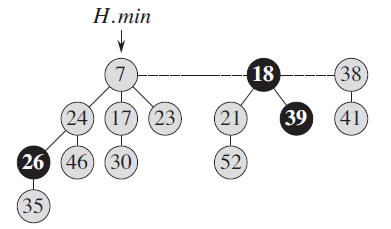
\includegraphics[width=\textwidth]{12_1}
		\label{fig:12.1}
	\end{figure}
	\item We have students $1, 2, \dots, n$ who need to be assigned to dormitories at a university that has an arbitrarily large number of dorms.
	There are $m$ same dormitory requests $(s_{1},t_{1}),(s_{2},t_{2}),\dots,(s_{m},t_{m})$ meaning students $s_{i}$ and $t_{i}$ must be assigned to the same dorm.
	There are also $k$ different dormitory requests $(u_{1},v_{1}),(u_{2},v_{2}),\dots,(u_{k},v_{k})$ meaning students $u_{i}$ and $t_{i}$ must be assigned to different dorms.
	Give an algorithm using the \Call{Union}{}-\Call{Find}{} structure to determine whether it is possible to assign students to forms so that all constraints are satisfied.
\end{enumerate}
%</Recitation-12>

\end{document}